\documentclass[11pt,twoside,a4paper,openright]{report}
%%%%%%%%%%%%%%%%%%%%%%%%%%%%%%%%%%%%%%%%%%%%%%%%
% Language, Encoding and Fonts
% http://en.wikibooks.org/wiki/LaTeX/Internationalization
%%%%%%%%%%%%%%%%%%%%%%%%%%%%%%%%%%%%%%%%%%%%%%%%
% Select encoding of your inputs. Depends on
% your operating system and its default input
% encoding. Typically, you should use
%   Linux  : utf8 (most modern Linux distributions)
%            latin1 
%   Windows: ansinew
%            latin1 (works in most cases)
%   Mac    : applemac
% Notice that you can manually change the input
% encoding of your files by selecting "save as"
% an select the desired input encoding. 
\usepackage[utf8]{inputenc}

% fancy tables
\usepackage{tabularx}

% Make latex understand and use the typographic
% rules of the language used in the document.
\usepackage[danish,english]{babel}
% Use the palatino font
\usepackage[sc]{mathpazo}
\linespread{1.05}         % Palatino needs more leading (space between lines)
% Choose the font encoding
\usepackage[T1]{fontenc}

%%%%%%%%%%%%%%%%%%%%%%%%%%%%%%%%%%%%%%%%%%%%%%%%
% Graphics and Tables
% http://en.wikibooks.org/wiki/LaTeX/Importing_Graphics
% http://en.wikibooks.org/wiki/LaTeX/Tables
% http://en.wikibooks.org/wiki/LaTeX/Colors
%%%%%%%%%%%%%%%%%%%%%%%%%%%%%%%%%%%%%%%%%%%%%%%%
% load a colour package
\usepackage[table,xcdraw]{xcolor}
\definecolor{aaublue}{RGB}{33,26,82}% dark blue
% The standard graphics inclusion package
\usepackage{graphicx}
% Set up how figure and table captions are displayed
\usepackage{caption}
\captionsetup{%
  font=footnotesize,% set font size to footnotesize
  labelfont=bf % bold label (e.g., Figure 3.2) font
}
% Make the standard latex tables look so much better
\usepackage{array,booktabs}
% Enable the use of frames around, e.g., theorems
% The framed package is used in the example environment
\usepackage{framed}

% Adds support for full page background picture
\usepackage[contents={},color=gray]{background}
%\usepackage[contents=draft,color=gray]{background}

%%%%%%%%%%%%%%%%%%%%%%%%%%%%%%%%%%%%%%%%%%%%%%%%
% Mathematics
% http://en.wikibooks.org/wiki/LaTeX/Mathematics
%%%%%%%%%%%%%%%%%%%%%%%%%%%%%%%%%%%%%%%%%%%%%%%%
% Defines new environments such as equation,
% align and split 
\usepackage{amsmath}
% Adds new math symbols
\usepackage{amssymb}
% Use theorems in your document
% The ntheorem package is also used for the example environment
% When using thmmarks, amsmath must be an option as well. Otherwise \eqref doesn't work anymore.
\usepackage[framed,amsmath,thmmarks]{ntheorem}

%Necessary for sub figures

\usepackage{graphicx}
\usepackage{subcaption}

%%%%%%%%%%%%%%%%%%%%%%%%%%%%%%%%%%%%%%%%%%%%%%%%
% Page Layout
% http://en.wikibooks.org/wiki/LaTeX/Page_Layout
%%%%%%%%%%%%%%%%%%%%%%%%%%%%%%%%%%%%%%%%%%%%%%%%

\usepackage{svg}
% Change margins, papersize, etc of the document
\usepackage[
  inner=28mm,% left margin on an odd page
  outer=41mm,% right margin on an odd page
  ]{geometry}
% Modify how \chapter, \section, etc. look
% The titlesec package is very configureable
\usepackage{titlesec}
\titleformat{\chapter}[display]{\normalfont\huge\bfseries}{\chaptertitlename\ \thechapter}{20pt}{\Huge}
\titleformat*{\section}{\normalfont\Large\bfseries}
\titleformat*{\subsection}{\normalfont\large\bfseries}
\titleformat*{\subsubsection}{\normalfont\normalsize\bfseries}
%\titleformat*{\paragraph}{\normalfont\normalsize\bfseries}
%\titleformat*{\subparagraph}{\normalfont\normalsize\bfseries}

% Clear empty pages between chapters
\let\origdoublepage\cleardoublepage
\newcommand{\clearemptydoublepage}{%
  \clearpage
  {\pagestyle{empty}\origdoublepage}%
}
\let\cleardoublepage\clearemptydoublepage

% Change the headers and footers
\usepackage{fancyhdr}
\pagestyle{fancy}
\fancyhf{} %delete everything
\renewcommand{\headrulewidth}{0pt} %remove the horizontal line in the header
\fancyhead[RE]{\small\nouppercase\leftmark} %even page - chapter title
\fancyhead[LO]{\small\nouppercase\rightmark} %uneven page - section title
\fancyhead[LE,RO]{\thepage} %page number on all pages
% Do not stretch the content of a page. Instead,
% insert white space at the bottom of the page
\raggedbottom
% Enable arithmetics with length. Useful when
% typesetting the layout.
\usepackage{calc}

%%%%%%%%%%%%%%%%%%%%%%%%%%%%%%%%%%%%%%%%%%%%%%%%
% Bibliography
% http://en.wikibooks.org/wiki/LaTeX/Bibliography_Management
%%%%%%%%%%%%%%%%%%%%%%%%%%%%%%%%%%%%%%%%%%%%%%%%
\usepackage[backend=bibtex,
  bibencoding=utf8,
  style=numeric-comp
  ]{biblatex}
\addbibresource{bib/mybib}

%%%%%%%%%%%%%%%%%%%%%%%%%%%%%%%%%%%%%%%%%%%%%%%%
% Misc
%%%%%%%%%%%%%%%%%%%%%%%%%%%%%%%%%%%%%%%%%%%%%%%%
% Add bibliography and index to the table of
% contents

\usepackage[nottoc]{tocbibind}
% Add the command \pageref{LastPage} which refers to the
% page number of the last page
\usepackage{lastpage}
% Add todo notes in the margin of the document
\usepackage[
%  disable, %turn off todonotes
  colorinlistoftodos, %enable a coloured square in the list of todos
  textwidth=\marginparwidth, %set the width of the todonotes
  textsize=scriptsize, %size of the text in the todonotes
  ]{todonotes}

%%%%%%%%%%%%%%%%%%%%%%%%%%%%%%%%%%%%%%%%%%%%%%%%
% Hyperlinks
% http://en.wikibooks.org/wiki/LaTeX/Hyperlinks
%%%%%%%%%%%%%%%%%%%%%%%%%%%%%%%%%%%%%%%%%%%%%%%%
% Enable hyperlinks and insert info into the pdf
% file. Hypperref should be loaded as one of the 
% last packages
\usepackage{hyperref}
\hypersetup{%
	pdfpagelabels=true,%
	plainpages=false,%
	pdfauthor={Author(s)},%
	pdftitle={Title},%
	pdfsubject={Subject},%
	bookmarksnumbered=true,%
	colorlinks=false,%
	citecolor=black,%
	filecolor=black,%
	linkcolor=black,% you should probably change this to black before printing
	urlcolor=black,%
	pdfstartview=FitH%
}
\usepackage{csquotes}

\usepackage{listings}

\usepackage{float}
\definecolor{codegreen}{rgb}{0,0.6,0}
\definecolor{codegray}{rgb}{0.5,0.5,0.5}
\definecolor{codepurple}{rgb}{0.58,0,0.82}
\definecolor{backcolour}{rgb}{0.95,0.95,0.92}
\definecolor{operatorblue}{HTML}{0000AA}
\definecolor{normaltextcolor}{HTML}{333333}

\lstdefinestyle{simpstyle}{
    backgroundcolor=\color{backcolour},   
    keywordstyle=[1]\color{magenta},
    keywordstyle=[2]\color{codepurple},
    %otherkeywordstyle=\color{blue},
    keywordstyle=[3]\color{operatorblue},
    numberstyle=\tiny\color{codegray},
    stringstyle=\color{codepurple},
    commentstyle=\color{codegreen},
    basicstyle=\color{normaltextcolor}\ttfamily\footnotesize,
    breakatwhitespace=false,         
    breaklines=true,                 
    captionpos=b,                    
    keepspaces=true,                 
    numbers=left,                    
    numbersep=5pt,                  
    showspaces=false,                
    showstringspaces=false,
    showtabs=false,                  
    tabsize=2
}

%\definecolor{operatorblue}{HTML}{0000AA}
%
%\lstdefinestyle{simpstyle}{
%    language=simp,
%    basicstyle = {\color{black}},
%    backgroundcolor = \color{Gray!20},
%    keywordstyle = {\color{teal}},
%    keywordstyle = [2]{\color{operatorblue}},
%    commentstyle = \color{purple}\bfseries,
%    stringstyle = \color{red}\bfseries,
%    otherkeywords = {;,.,\,,\(,\),\{,\},\[,\],=,:,!,>,<,-,+,*,/,\%},
%    morekeywords = [2]{;,.,\,,\(,\),\{,\},\[,\],=,:,!,>,<,-,+,*,/,\%},
%}

\lstdefinelanguage{simp}{
    morekeywords={[1]Rules, Units, Board, Cell, Events, Init, if, else, return, Turn, Unit, Game, Players},
    morekeywords={[2]AND, OR, XOR, bool, int, string, double, float, true, false, this},
    sensitive=true,
    comment=[l]{//},
    morecomment=[s]{/*}{*/},
    morestring=[b]',
    morestring=[b]"
}[keywords]

\usepackage{wrapfig}
% package inclusion and set up of the document
% see, e.g., http://en.wikibooks.org/wiki/LaTeX/Formatting#Hyphenation
% for more information on word hyphenation
\hyphenation{ex-am-ple hy-phen-a-tion short}
\hyphenation{long la-tex}
% 
% see, e.g., http://en.wikibooks.org/wiki/LaTeX/Customizing_LaTeX#New_commands
% for more information on how to create macros

%%%%%%%%%%%%%%%%%%%%%%%%%%%%%%%%%%%%%%%%%%%%%%%%
% Macros for the titlepage
%%%%%%%%%%%%%%%%%%%%%%%%%%%%%%%%%%%%%%%%%%%%%%%%
%Creates the aau titlepage
\newcommand{\aautitlepage}[3]{%
  {
    %set up various length
    \ifx\titlepageleftcolumnwidth\undefined
      \newlength{\titlepageleftcolumnwidth}
      \newlength{\titlepagerightcolumnwidth}
    \fi
    \setlength{\titlepageleftcolumnwidth}{0.5\textwidth-\tabcolsep}
    \setlength{\titlepagerightcolumnwidth}{\textwidth-2\tabcolsep-\titlepageleftcolumnwidth}
    %create title page
    \thispagestyle{empty}
    \noindent%
    \begin{tabular}{@{}ll@{}}
      \parbox{\titlepageleftcolumnwidth}{
        \iflanguage{danish}{%
          
\includegraphics[width=\titlepageleftcolumnwidth]{AAUgraphics/aau_logo_da}
        }{%
          
\includegraphics[width=\titlepageleftcolumnwidth]{AAUgraphics/aau_logo_en}
        }
      } &
      \parbox{\titlepagerightcolumnwidth}{\raggedleft\sf\small
        #2
      }\bigskip\\
       #1 &
      \parbox[t]{\titlepagerightcolumnwidth}{%
      \textbf{Abstract:}\bigskip\par
        \fbox{\parbox{\titlepagerightcolumnwidth-2\fboxsep-2\fboxrule}{%
          #3
        }}
      }\\
    \end{tabular}
    \vfill
    \iflanguage{danish}{%
      \noindent{\footnotesize\emph{Rapportens indhold er frit tilgængeligt, men offentliggørelse (med kildeangivelse) må kun ske efter aftale med forfatterne.}}
    }{%
      \noindent{\footnotesize\emph{The content of this report is freely available, but publication (with reference) may only be pursued due to agreement with the author.}}
    }
    \clearpage
  }
}

%Create english project info
\newcommand{\englishprojectinfo}[8]{%
  \parbox[t]{\titlepageleftcolumnwidth}{
    \textbf{Title:}\\ #1\bigskip\par
    \textbf{Theme:}\\ #2\bigskip\par
    \textbf{Project Period:}\\ #3\bigskip\par
    \textbf{Project Group:}\\ #4\bigskip\par
    \textbf{Participant(s):}\\ #5\bigskip\par
    \textbf{Supervisor(s):}\\ #6\bigskip\par
    \textbf{Copies:} #7\bigskip\par
    \textbf{Page Numbers:} \pageref{LastPage}\bigskip\par
    \textbf{Date of Completion:}\\ #8
  }
}

%Create danish project info
\newcommand{\danishprojectinfo}[8]{%
  \parbox[t]{\titlepageleftcolumnwidth}{
    \textbf{Titel:}\\ #1\bigskip\par
    \textbf{Tema:}\\ #2\bigskip\par
    \textbf{Projektperiode:}\\ #3\bigskip\par
    \textbf{Projektgruppe:}\\ #4\bigskip\par
    \textbf{Deltager(e):}\\ #5\bigskip\par
    \textbf{Vejleder(e):}\\ #6\bigskip\par
    \textbf{Oplagstal:} #7\bigskip\par
    \textbf{Sidetal:} \pageref{LastPage}\bigskip\par
    \textbf{Afleveringsdato:}\\ #8
  }
}

%%%%%%%%%%%%%%%%%%%%%%%%%%%%%%%%%%%%%%%%%%%%%%%%
% An example environment
%%%%%%%%%%%%%%%%%%%%%%%%%%%%%%%%%%%%%%%%%%%%%%%%
\theoremheaderfont{\normalfont\bfseries}
\theorembodyfont{\normalfont}
\theoremstyle{break}
\def\theoremframecommand{{\color{gray!50}\vrule width 5pt \hspace{5pt}}}
\newshadedtheorem{exa}{Example}[chapter]
\newenvironment{example}[1]{%
		\begin{exa}[#1]
}{%
		\end{exa}
}
% my new macros

\begin{document}
%frontmatter
\pagestyle{empty} %disable headers and footers
\pagenumbering{roman} %use roman page numbering in the frontmatter
%\pdfbookmark[0]{Front page}{label:frontpage}%

\begin{titlepage}
\newgeometry{top=0cm,bottom=1.2cm,right=0cm,left=0cm}

  \backgroundsetup{
   scale=1.1,
   angle=0,
   opacity=1.0,  %% adjust
   contents={\includegraphics[width=\paperwidth,height=\paperheight]{AAUgraphics/aau_waves}}
    }
		
  \begin{center} %%please do not change the height or width of the frontpage image
    \centerline{
\includegraphics[totalheight=0.5\paperwidth,width=1\paperwidth]{AAUgraphics/frontpageImage}}% 
  \end{center}
	
	\vspace*{-0.96cm}
  {\noindent\color{aaublue}\fboxsep0pt\colorbox{white}{\begin{tabular}{@{}p{\paperwidth}@{}}
    \centerline{
    \begin{minipage}{0.85\textwidth}
        \bigskip
				\bigskip
        \centering
        \Huge{\textbf{
A simple explanation of how our Universe was formed% insert your title here
        }}
    \end{minipage}
    }
		
	\centerline{
	\begin{minipage}{0.9\textwidth}
        \bigskip
        \centering
        \Large{
Development of a predictive model% insert your subtitle here
        }
    \end{minipage}
    }
			
	\centerline{
	\begin{minipage}{0.9\textwidth}
        \bigskip
        \centering
        {\Large
Anders Andersen, Alfred Alfredsen, Anne Annesen% insert names separated by comma
        }
    \end{minipage}
    }
			
    \centerline{
    \begin{minipage}{0.9\textwidth}
        \bigskip
        \centering
        {\large
Energy Technology, TEPE4-1005, \the\year-06% insert name of study, group number, year-month
        } 
    \end{minipage}
    }
			
    \centerline{
    \begin{minipage}{0.9\textwidth}
        \bigskip
        \centering
%% Comment this section if you are not doing Bachelor or Master Project   
        {\Large
Master's Project
      %Bachelor Project
        }
        \smallskip
    \end{minipage}
    }
			
  \end{tabular}}}

  \vfill
  \begin{figure}[!b]
	\centering
    
\includegraphics[width=0.2\paperwidth]{AAUgraphics/aau_logo_circle_en}% comment this line in for English version
    %
\includegraphics[width=0.2\paperwidth]{AAUgraphics/aau_logo_circle_da} %comment this line in for Danish version
  \end{figure}
\end{titlepage}
\restoregeometry
\pdfbookmark[0]{Front page}{label:frontpage}%
\begin{titlepage}
\vspace*{\fill}
    \backgroundsetup{
    scale=1.1,
    angle=0,
    opacity=1.0,  %% adjust
    contents={\includegraphics[width=\paperwidth,height=\paperheight]{AAUgraphics/aau_waves}}
    }
  \addtolength{\hoffset}{0.5\evensidemargin-0.5\oddsidemargin} %set equal margins on the frontpage - remove this line if you want default margins
  \noindent%
  {\color{white}\fboxsep0pt\colorbox{aaublue}{\begin{tabular}{@{}p{\textwidth}@{}}
    \begin{center}
    \Huge{\textbf{
      FSL placeholder% insert your title here
    }}
    \end{center}
    \begin{center}
      \Large{
        Generating Music Using Machine Learning% insert your subtitle here
      }
    \end{center}
    \vspace{0.2cm}
   \begin{center}
    {\Large
      Emil Dalgaard Moroder, Fatemeh Shad Bakhsh, Iñigo Sanz Ilundain, Jan Mackeprang Damgaard Hansen, Kristian Skov Johansen, Nicholas Herrmann% insert names separated by comma
    }\\
    \vspace{0.2cm}
    {\large
      Computer Science, \today % insert name of study, group number, year-month
    }
   \end{center}
   \vspace{0.2cm}
%% Comment this section in if you are doing Bachelor or Master Project   
   \begin{center}
    {\Large
      8th Semester Project
    }
   \end{center}
  \end{tabular}}}
  \vfill
  \begin{center}
    
\includegraphics[width=0.2\paperwidth]{AAUgraphics/aau_logo_circle_en}% comment this line in for English version
    %
\includegraphics[width=0.2\paperwidth]{AAUgraphics/aau_logo_circle_da} %comment this line in for Danish version
  \end{center}
\end{titlepage}
\clearpage

\thispagestyle{empty}
{\small
\strut\vfill % push the content to the bottom of the page
\noindent Copyright \copyright{} Aalborg University 2023\par
\vspace{0.2cm}
\noindent 
}
\clearpage


\pdfbookmark[0]{English title page}{label:titlepage_en}
\aautitlepage{%
  \englishprojectinfo{
    Title %title
  }{%
    Theme %theme
  }{%
    Spring Semester 2023 %project period
  }{%
    cs-23-dat-8-07 % project group
  }{%
    %list of group members
    Emil Dalgaard Moroder\\ 
    Fatemeh Shad Bakhsh\\
    Iñigo Sanz Ilundain\\
    Jan Mackeprang Damgaard Hansen\\
    Kristian Skov Johansen\\
    Nicholas Herrmann\\
  }{%
    %list of supervisors
    Nguyen Thi Thao Ho
  }{%
    1 % number of printed copies
  }{%
    \today % date of completion
  }%
}{%department and address
  \textbf{Computer Science}\\
  Aalborg University\\
  \href{http://www.cs.aau.dk}{http://www.cs.aau.dk}
}{% the abstractNguyen Thi Thao Ho
}
\cleardoublepage
\pdfbookmark[0]{Contents}{label:contents}
\pagestyle{fancy} %enable headers and footers again
\tableofcontents
\chapter*{Preface\markboth{Preface}{Preface}}\label{ch:preface}
\addcontentsline{toc}{chapter}{Preface}
%Here is the preface. You should put your signatures at the end of the preface.
The group's members extend their gratitude to Nguyen Thi Thao Ho for her supervision and guidance.
% 

\vspace{\baselineskip}\hfill Aalborg University, \today
\vfill\noindent
\begin{minipage}[b]{0.45\textwidth}
 \centering
 \rule{\textwidth}{0.5pt}\\
  Emil Dalgaard Moroder\\
 {\footnotesize <emorod19@student.aau.dk>}
\end{minipage}
\hfill
\begin{minipage}[b]{0.45\textwidth}
 \centering
 \rule{\textwidth}{0.5pt}\\
  Fatemeh Shad Bakhsh\\
 {\footnotesize <bakhs22@student.aau.dk>}
\end{minipage}
\vfill\noindent
\begin{minipage}[b]{0.45\textwidth}
 \centering
 \rule{\textwidth}{0.5pt}\\
  Iñigo Sanz Iludain\\
 {\footnotesize <isanzi22@student.aau.dk>>}
\end{minipage}
\hfill
\begin{minipage}[b]{0.45\textwidth}
 \centering
 \rule{\textwidth}{0.5pt}\\
  Jan Mackeprang Damgaard Hansen\\
 {\footnotesize <jmdh19@student.aau.dk>}
\end{minipage}
\vfill\noindent
\begin{minipage}[b]{0.45\textwidth}
 \centering
 \rule{\textwidth}{0.5pt}\\
  Kristian Skov Johansen\\\
 {\footnotesize <kjohan19@student.aau.dk>}
\end{minipage}
\hfill
\begin{minipage}[b]{0.45\textwidth}
 \centering
 \rule{\textwidth}{0.5pt}\\
  Nicholas Herrmann\\
 {\footnotesize <nherrm19@student.aau.dk>}
\end{minipage}
\vspace{3\baselineskip}
\cleardoublepage
%mainmatter
\pagenumbering{arabic} %use arabic page numbering in the mainmatter
\chapter{Introduction}



\chapter{Preliminaries and Related Work}
\section{Time Series}
%introduction

\subsection{Time Series Data}
Time series data are sequences of data collected over and ordered by time. A common example is a data set consisting of the hourly energy consumption of a household, as shown in table \ref{tab:hourlyEnergyConsumption}. Here, each piece of data is a measurement of the amount of energy consumed throughout the past hour. As in the example above, time series data sets usually consist of data points which are collected at equal time intervals. In the example above, there is only one dependent variable; the consumption, which is dependent on the time. Time series with this characteristic are called \emph{univariate}. Had there been multiple dependent variables, the time series would be \emph{multivariate}.
%

\begin{table}[]

\begin{tabular}{l|lllllllllll}
\rowcolor[HTML]{EFEFEF} 
\textbf{t}                                                  & \textbf{13:00} & \textbf{14:00} & \textbf{15:00} & \textbf{16:00} & \textbf{17:00} & \textbf{18:00} & \textbf{19:00} & \textbf{20:00} & \textbf{21:00} & \textbf{22:00}  \\ \hline
\begin{tabular}[c]{@{}l@{}}Consumption\\ (kWh)\end{tabular} & 0.10           & 0.17           & 0.15           & 0.21           & 0.20           & 0.25           & 0.15           & 0.20           & 0.28           & 0.15                     
\end{tabular}
\caption{Time series of hourly energy consumption of a household, measured in kWh.}
\label{tab:hourlyEnergyConsumption}
\end{table}


\subsection{Time Series Analysis}
Time series are common in computer science, and therefore, a number of analysis methods have been devised. One pattern which is common in time series analysis is to divide the time series up into subsequences, and apply a function to each subsequence in order to extract information from it. This technique is called \emph{sliding window}, since it can be thought of as sliding a window across the sequence, and applying the function to what is visible through the window. 

A common first step when analysing time series is to use a sliding window with an averaging function to denoise the data. For instance, using a sliding window of size 3 on the time series shown in table \ref{tab:hourlyEnergyConsumption}, and averaging the data points in the window yields the smoothed time series shown in figure \ref{fig:slidingWindowIllustration}.

\begin{figure}
    \centering
    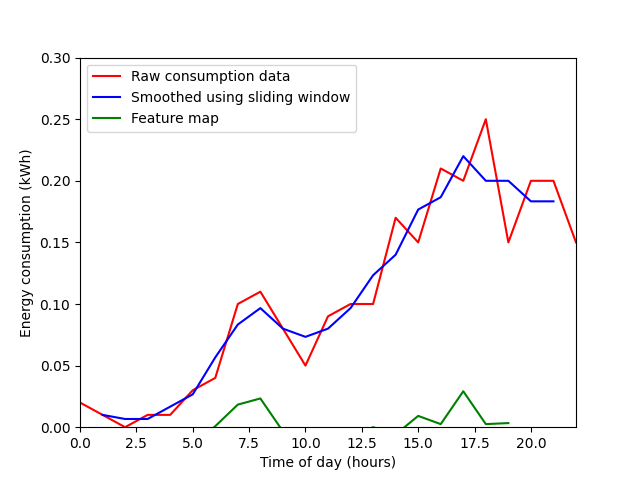
\includegraphics[scale=0.5]{img/prerequisites/energyConsumptionPlots.png}
    \caption{Effect of using a sliding window of size 3 with the averaging function to reduce noise in time series data, and feature map found by applying the kernel $\begin{bmatrix}-0.125 & -0.125 & 0.5 & -0.125 & -0.125 \end{bmatrix}$ to the smoothed data. For the feature map, the $y$-axis represents how well the given window matches the pattern defined by the kernel.}
    \label{fig:slidingWindowIllustration}
\end{figure}

Aplying a sliding window with an averaging function is a useful preprocessing step, but sliding windows can also be used to do actual analysis. A common operation to apply when using sliding windows for analysis is convolution.

\subsubsection{Convolutions for time series analysis}
In the context of vectors of finite length, the convolution operation is a method for assessing the presence of a pattern in a vector. Formally, the convolution operation is defined as follows\footnote{This is actually the cross-correlation operation, but in a machine learning context, the two operations are used interchangeably}:

\begin{equation}\label{eq:1dconvolution}
    [\boldsymbol{w} \circledast \boldsymbol{x}]i = \sum_u^{L-1} w_u x_{i+u}
\end{equation}

where $\boldsymbol{w}$ is a the weight vector, which defines the pattern to detect, $\boldsymbol{x}$ is the vector to be analysed, and $L$ is the length of $\boldsymbol{w}$. $\boldsymbol{w}$ is called the \emph{kernel}, and the output of the convolution is called the \emph{feature map}. One can then imagine sliding $\boldsymbol{w}$ across an input vector $\boldsymbol{x}$ which is longer than $\boldsymbol{w}$ to see where in $\boldsymbol{x}$ the pattern defined by $\boldsymbol{w}$ is present. An illustration of this is shown in figure \ref{fig:slidingWindowIllustration}. Here, the kernel $\begin{bmatrix}-0.125 & -0.125 & 0.5 & -0.125 & -0.125 \end{bmatrix}$ is applied to the smoothed energy consumption data. Intuitively, this kernel finds instances of peaks; it rewards high values in the center of the window, and penalises high values in the edges. Using this kernel, we were able to identify two peaks; one in the morning and one in the afternoon. Of course, convolution can be used to identify much more complex patterns than peaks. Ideally, one would have a machine learning model learn which patterns are the most useful, and learn the kernels which capture them.

Equation \ref{eq:1dconvolution} shows how to apply the convolution operation to a one-dimensional vector. This is useful when analysing univariate time series, but for multivariate time series we may want to find patterns between variables. In this case, we can define a two dimensional kernel $\mathbf{W}$, and define the convolution operation as follows:

\begin{equation}\label{eq:2dconvolution}
    [\mathbf{W} \circledast \mathbf{X}]_{i,j} = \sum_u^W \sum_v^H w_{u,v}x_{i+u,j+v}
\end{equation}
where $\mathbf{W}\in \mathbb{R}^{W\times H}$.

%pros, cons

\subsubsection{Shapelets}
%pros, cons

\section{Few Shot Learning}
%What to expect
This section will explain what \textit{Few Shot Learning (FSL)} is, and why FSL has seen a considerable amount of interest. Furthermore, it will present relevant terminology and different approaches to solving the problem of FSL.

%Motivation + general overview
Conventional machine learning models have been shown to be highly accurate at classification and regression. However, the problem is that these models require immense datasets to be effective, and as a result the smaller the dataset the worse the result. FSL tries to solve the problem of being accurate on small datasets by using prior knowledge, which makes it able to generalise on new tasks on only a few data samples \cite{fsl2019}.

%Introduction to FSL
Humans are capable of quickly applying previously learned information to a new task, e.g. a child that has never seen the number "1" \textit{Query} before, is able to classify what class it belongs by only using other numbers \textit{(Support Set)}. This is illustrated in the \ref{fig:query_support}, where the child is given a picture of the number "1", and a support set of five other numbers which include the query class. The child is able to successfully identify which of the five classes is the same as the query class by using his prior knowledge. The number of classes in the support set is known as N-way, and the number of samples of each class is the K-shot. This is typically known as N-way-K-Shot classification. As one can imagine from the given example, the more K-shots the child has the easier it might be to classify, and the larger the N-way, the harder it is, since some classes might share similarities which could result in a wrong classification. Additionally, if one has to predict a query class and has support sets $|S_1| = 5$ and $|S_2| = 10$, and one picks a random class the probability of a correct guess is respectively, $20\%$ and $10\%$. Hereafter, we will introduce FSL in a more formal manner.

%Formal introduction 
Moreover, given a learning task $\mathcal{T}$ and a dataset $\mathcal{D}=\{\mathcal{D}_{train}, \mathcal{D}_{test}\}$. The training set is defined as $\mathcal{D}_{train} = \{{(x_i, y_i)}\}^{I}_{i=1}$, where I is very small compoared to traditional datasets. The test set is defined as $\mathcal{D}_{test}=\{x^{test}\}$
 

\begin{figure}
    \centering
    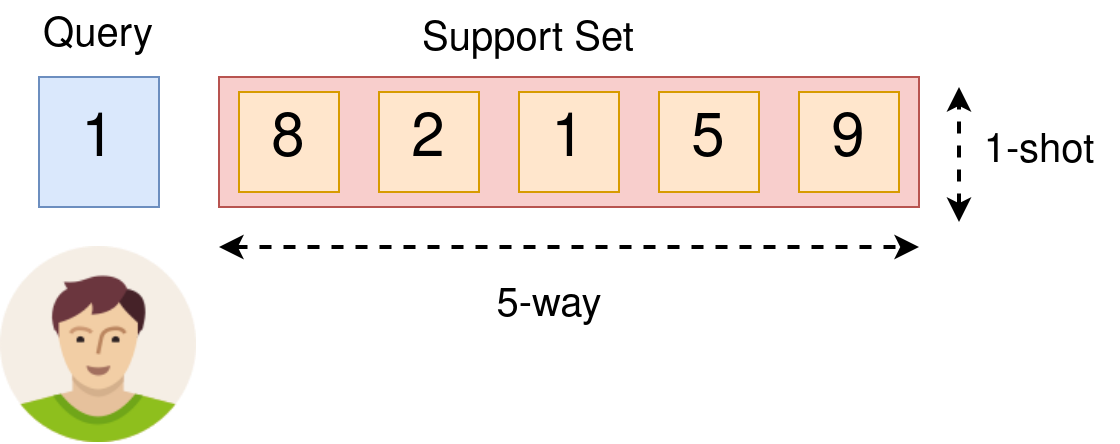
\includegraphics[scale=0.25]{img/prerequisites/query_support.png}
    \caption{Few shot learning example}
    \label{fig:query_support}
\end{figure}



\subsubsection{Protonets}


\subsection{Interpretability}
The following segment will provide an overview of interpretability and elucidate why it is a topic that has seen interest in the context of machine learning.

%Short overview
The concepts of \textit{artificial intelligence (ai)} and \textit{machine learning (ML)} are often seen as intimidating black box models that cannot be understood by the general public. Through various techniques, interoperability tries to explain the black-box models into a domain that the general public can understand.


\subsection{Embedding}
% If you do not write the report in English, translating the bibliography title to, e.g., Danish, should not be done here. Instead, you should change the main language in the preamble (look for the line \usepackage[danish,english]{babel} and change the order/delete the 'english' option). See more in the babel package documentation.
\printbibliography[heading=bibintoc, title=Bibliography]
\label{bib:mybiblio}
\appendix
\end{document}
